\documentclass{report}
\usepackage{graphicx}
\usepackage{verbatim}
\usepackage{pgfplots}
\usepackage{circuitikz}
\usepackage{amsmath}
\graphicspath{ {./images/} }
\title{P01 Report}
\author{Vijay Anant }
\date{February 2019}

\begin{document}
\maketitle
\chapter{Theoretical part}
\begin{center}
    
\begin{circuitikz} \draw

    

(0,0) to[battery] (0,4)
  to[resistor] (4,4) -- (4,0)
  to[resistor] (0,0)
;

\end{circuitikz}


Electrical Circuit Diagram
\end{center}


\section{Circuit Calculation}
Theoretical calculation of the
circuit
V1=12.5V
R1=3ohm
R2=6ohm
VR = (R x VT) / RT
VR1=  (R1 x V1) / RT = 12.5 V
VR2= (R2 x V2)/ RT = 8.333 V



\begin{figure}[hbt!]
\begin{center}
\begin{tabular}{ |c|c| } 
 \hline
 V1 & 12.5V  \\ 
 R1 & 3ohm  \\ 
 R2 & 6ohm \\
 UR1 & 12.5V  \\ 
 UR2 & 8.33V \\
 \hline
\end{tabular}
\end{center}
 \end{figure}
 \begin{center}
\begin{tikzpicture}
\begin{axis}[axis lines = left,
    xlabel = $f(R2)$,
    ylabel = $U(R2)$ ]
    \addplot [black, very thick]{x*1/x};
    
\end{axis}
\end{tikzpicture}
\end{center}

\chapter{Practical part}
Practical Calculation
\section{‘Work with GEDA programs'}
\subsection{'Work with gschem'}
\begin{figure}[hbt!]
 \centering
 \caption{Circuit Diagram createed in gscehm}
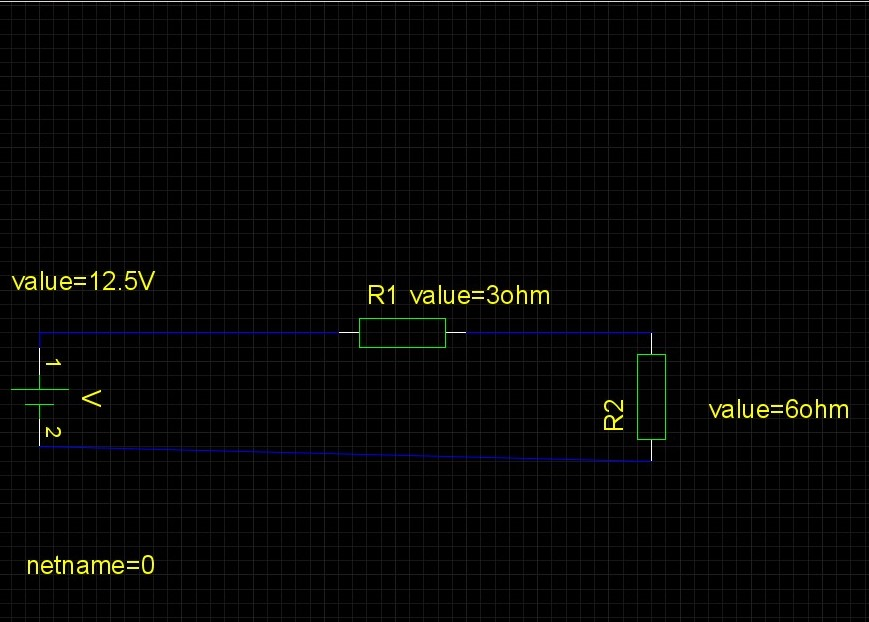
\includegraphics[width=\textwidth]{01.jpg}
 \end{figure}
\subsection{'Work with gnetlist'}


\subsection{'Work with ngspice'}
\begin{figure}[hbt!]
 \centering
  \caption{The plotted graph after using ngspice}
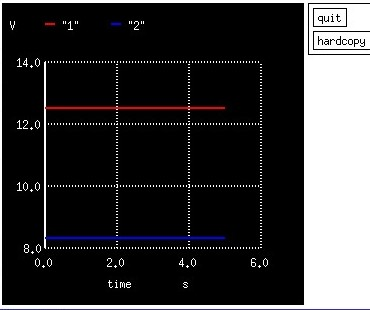
\includegraphics[width=\textwidth]{02.jpg}
 \end{figure}


\section{‘‘Work with QUCS programs'}

Image of Schematics
\begin{figure}[hbt!]
 \centering
 \caption{Circuit Diagram in QUCS}
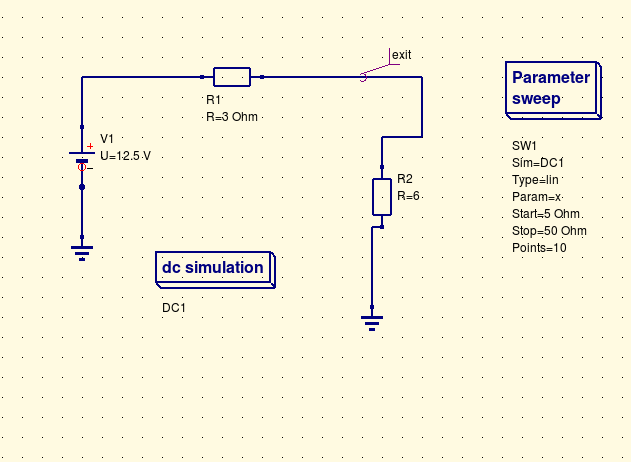
\includegraphics[width=\textwidth]{03.png}
 \end{figure}
 
DC simulation
\begin{figure}[hbt!]
 \centering
 \caption{DC Simulation}
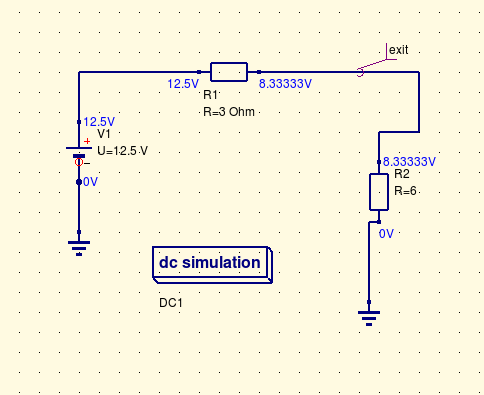
\includegraphics[width=\textwidth]{05.png}
 \end{figure}
 
 

Curve and Table obtained from DC Simulation

 
\begin{figure}[hbt!]
 \centering
 \caption{The following graph shows the DC simulation for the various obtained values}
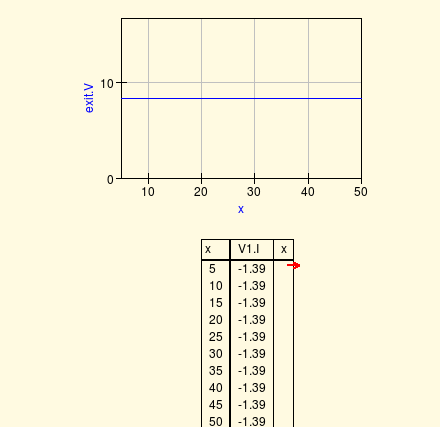
\includegraphics[width=\textwidth]{06.png}
 \end{figure}

\begin{figure}[hbt!]
 \centering
  \caption{The following graph shows the Sweep Simulation for the various obtained values}
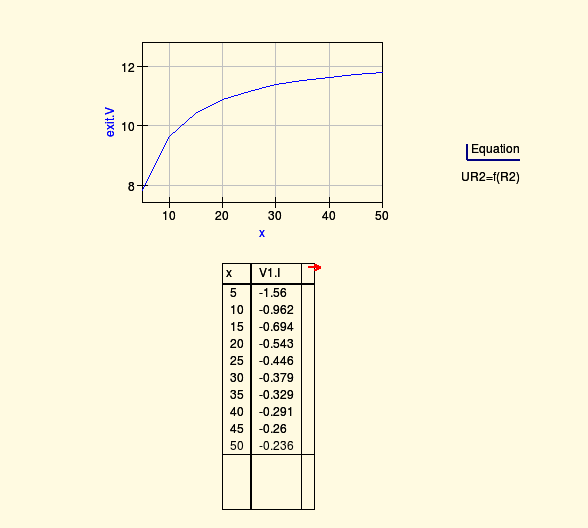
\includegraphics[width=\textwidth]{04.png}

\end{figure}
\end{document}
